\section{Results}
\label{sec:results}

All arms of a run share the checkpoint, the fold, the seed, the test epochs
and the probe subsample, so every comparison below is paired. Reported
differences are means of per-run differences with a $95\%$ confidence
interval and a two-sided Wilcoxon $p$-value; $n$ is the number of paired runs.
Tables~\ref{tab:main-eegnet} and~\ref{tab:main-sleepcnn} collect the arm means
for the four settings of each backbone, and Table~\ref{tab:pairs} collects the
key paired contrasts. ``Probe'' is the subject-identification accuracy of a
linear readout of the penultimate representation, ``within'' is the same probe
refitted inside each stage and averaged over stages, and chance is $0.25$ for
the four held-out patients of a Sleep-EDF fold and $1/31\approx0.032$ for the
thirty-one recordings of an HMC fold. ``$\kappa$'', ``MF1'' and ``ECE'' are
Cohen's $\kappa$, the macro-averaged $F_1$ and the expected calibration error
of the posterior. ``Worst'' and ``SD'' are the minimum and
the standard deviation of per-patient conformal coverage at $\alpha=0.1$.

\begin{table*}[t]
\centering
\caption{EEGNet: mean over runs per arm (five folds $\times$ three seeds on
Sleep-EDF, five folds $\times$ two seeds on HMC). ``Probe'' and ``Within'' are
subject identification overall and within stage; ``$\kappa$'' and ``MF1'' are
Cohen's $\kappa$ and the macro-averaged $F_1$; ``ECE'' is the expected
calibration error; ``Worst'' and ``SD'' are the
minimum and standard deviation of per-patient conformal coverage at
$\alpha=0.1$. Standard AdaBN and the batch-normalization Tent procedure are
not applicable to group-normalized checkpoints and are omitted there.}
\label{tab:main-eegnet}
\resizebox{\textwidth}{!}{\begin{tabular}{llrrrrrrrrr}
\toprule
Cohort & Arm & $n$ & Acc & $\kappa$ & MF1 & ECE & Probe & Within & Worst & SD \\
\midrule
Sleep-EDF BN & BN & 15 & 0.781 & 0.698 & 0.644 & 0.030 & 0.715 & 0.738 & 0.828 & 0.055 \\
 & Marginal & 15 & 0.777 & 0.686 & 0.642 & 0.033 & 0.301 & 0.735 & 0.838 & 0.047 \\
 & AdaBN & 15 & 0.782 & 0.696 & 0.645 & 0.043 & 0.466 & 0.700 & 0.866 & 0.028 \\
 & SCSN & 15 & 0.784 & 0.701 & 0.645 & 0.044 & 0.314 & 0.465 & 0.857 & 0.036 \\
 & SCSN-$\lambda_{0.5}$ & 15 & 0.788 & 0.707 & 0.648 & 0.034 & 0.529 & 0.598 & 0.845 & 0.043 \\
 & Tent-SGD & 15 & 0.782 & 0.698 & 0.647 & 0.038 & 0.384 & 0.714 & 0.870 & 0.023 \\
\addlinespace
HMC BN & BN & 10 & 0.672 & 0.564 & 0.594 & 0.028 & 0.385 & 0.527 & 0.649 & 0.086 \\
 & Marginal & 10 & 0.648 & 0.522 & 0.571 & 0.035 & 0.074 & 0.411 & 0.599 & 0.096 \\
 & AdaBN & 10 & 0.674 & 0.563 & 0.591 & 0.029 & 0.212 & 0.473 & 0.698 & 0.069 \\
 & SCSN & 10 & 0.690 & 0.587 & 0.613 & 0.033 & 0.073 & 0.209 & 0.678 & 0.067 \\
 & SCSN-$\lambda_{0.5}$ & 10 & 0.689 & 0.586 & 0.610 & 0.034 & 0.205 & 0.340 & 0.680 & 0.072 \\
 & Tent-SGD & 10 & 0.680 & 0.570 & 0.597 & 0.025 & 0.179 & 0.453 & 0.673 & 0.070 \\
\addlinespace
Sleep-EDF GN & BN & 15 & 0.770 & 0.683 & 0.634 & 0.041 & 0.541 & 0.638 & 0.855 & 0.038 \\
 & Marginal & 15 & 0.778 & 0.690 & 0.637 & 0.031 & 0.298 & 0.616 & 0.863 & 0.029 \\
 & AdaBN & -- & -- & -- & -- & -- & -- & -- & -- & -- \\
 & SCSN & 15 & 0.780 & 0.696 & 0.640 & 0.044 & 0.330 & 0.449 & 0.864 & 0.034 \\
 & SCSN-$\lambda_{0.5}$ & -- & -- & -- & -- & -- & -- & -- & -- & -- \\
 & Tent-SGD & -- & -- & -- & -- & -- & -- & -- & -- & -- \\
\addlinespace
HMC GN & BN & 10 & 0.693 & 0.595 & 0.628 & 0.026 & 0.231 & 0.369 & 0.695 & 0.067 \\
 & Marginal & 10 & 0.697 & 0.593 & 0.632 & 0.017 & 0.057 & 0.315 & 0.724 & 0.059 \\
 & AdaBN & -- & -- & -- & -- & -- & -- & -- & -- & -- \\
 & SCSN & 10 & 0.709 & 0.616 & 0.643 & 0.017 & 0.065 & 0.156 & 0.708 & 0.059 \\
 & SCSN-$\lambda_{0.5}$ & -- & -- & -- & -- & -- & -- & -- & -- & -- \\
 & Tent-SGD & -- & -- & -- & -- & -- & -- & -- & -- & -- \\
\bottomrule
\end{tabular}
}
\end{table*}

\begin{table*}[t]
\centering
\caption{SleepCNN, same layout as Table~\ref{tab:main-eegnet}; Sleep-EDF
SleepCNN uses one seed per fold (five runs per arm) and HMC uses two (ten
runs per arm).}
\label{tab:main-sleepcnn}
\resizebox{\textwidth}{!}{\begin{tabular}{llrrrrrrrrr}
\toprule
Cohort & Arm & $n$ & Acc & $\kappa$ & MF1 & ECE & Probe & Within & Worst & SD \\
\midrule
Sleep-EDF BN & BN & 5 & 0.803 & 0.730 & 0.709 & 0.038 & 0.847 & 0.848 & 0.840 & 0.048 \\
 & Marginal & 5 & 0.805 & 0.729 & 0.696 & 0.024 & 0.298 & 0.865 & 0.870 & 0.028 \\
 & AdaBN & 5 & 0.814 & 0.738 & 0.719 & 0.029 & 0.773 & 0.848 & 0.869 & 0.025 \\
 & SCSN & 5 & 0.800 & 0.725 & 0.699 & 0.043 & 0.319 & 0.550 & 0.847 & 0.034 \\
 & SCSN-$\lambda_{0.5}$ & 5 & 0.805 & 0.732 & 0.707 & 0.037 & 0.634 & 0.694 & 0.845 & 0.040 \\
 & Tent-SGD & 5 & 0.818 & 0.746 & 0.715 & 0.026 & 0.766 & 0.858 & 0.871 & 0.023 \\
\addlinespace
HMC BN & BN & 10 & 0.698 & 0.598 & 0.641 & 0.034 & 0.681 & 0.805 & 0.645 & 0.075 \\
 & Marginal & 10 & 0.663 & 0.541 & 0.602 & 0.068 & 0.126 & 0.720 & 0.711 & 0.061 \\
 & AdaBN & 10 & 0.702 & 0.598 & 0.647 & 0.030 & 0.324 & 0.723 & 0.649 & 0.072 \\
 & SCSN & 10 & 0.712 & 0.615 & 0.654 & 0.036 & 0.090 & 0.374 & 0.664 & 0.066 \\
 & SCSN-$\lambda_{0.5}$ & -- & -- & -- & -- & -- & -- & -- & -- & -- \\
 & Tent-SGD & -- & -- & -- & -- & -- & -- & -- & -- & -- \\
\addlinespace
Sleep-EDF GN & BN & 5 & 0.806 & 0.732 & 0.709 & 0.026 & 0.821 & 0.832 & 0.860 & 0.035 \\
 & Marginal & 5 & 0.816 & 0.744 & 0.715 & 0.021 & 0.295 & 0.889 & 0.864 & 0.029 \\
 & AdaBN & -- & -- & -- & -- & -- & -- & -- & -- & -- \\
 & SCSN & 5 & 0.817 & 0.747 & 0.718 & 0.035 & 0.323 & 0.583 & 0.870 & 0.025 \\
 & SCSN-$\lambda_{0.5}$ & -- & -- & -- & -- & -- & -- & -- & -- & -- \\
 & Tent-SGD & -- & -- & -- & -- & -- & -- & -- & -- & -- \\
\addlinespace
HMC GN & BN & 10 & 0.719 & 0.627 & 0.665 & 0.025 & 0.528 & 0.663 & 0.677 & 0.070 \\
 & Marginal & 10 & 0.698 & 0.593 & 0.641 & 0.031 & 0.122 & 0.745 & 0.724 & 0.058 \\
 & AdaBN & -- & -- & -- & -- & -- & -- & -- & -- & -- \\
 & SCSN & 10 & 0.728 & 0.639 & 0.674 & 0.025 & 0.088 & 0.341 & 0.697 & 0.059 \\
 & SCSN-$\lambda_{0.5}$ & -- & -- & -- & -- & -- & -- & -- & -- & -- \\
 & Tent-SGD & -- & -- & -- & -- & -- & -- & -- & -- & -- \\
\bottomrule
\end{tabular}
}
\end{table*}

\begin{table}[t]
\centering
\caption{Paired differences for the key contrasts, with the Wilcoxon
$p$-value in parentheses. Upper block: accuracy. Lower block: within-stage
subject probe. A negative probe difference means less identity.}
\label{tab:pairs}
\small
\resizebox{\columnwidth}{!}{\begin{tabular}{lcccc}
\toprule
Contrast & \shortstack{edf\\bn\\eegnet} & \shortstack{edf\\bn\\sleepcnn} & \shortstack{hmc\\bn\\eegnet} & \shortstack{hmc\\bn\\sleepcnn} \\
\midrule
\multicolumn{5}{l}{\emph{Accuracy difference}} \\
SCSN $-$ BN & +0.002 (0.359) & -0.004 (0.812) & +0.019 (0.00195) & +0.014 (0.00391) \\
SCSN $-$ Marginal & +0.007 (0.252) & -0.005 (0.812) & +0.042 (0.00195) & +0.049 (0.00195) \\
SCSN $-$ AdaBN & +0.002 (0.89) & -0.014 (0.812) & +0.016 (0.00195) & +0.010 (0.084) \\
AdaBN $-$ BN & +0.001 (0.804) & +0.010 (0.625) & +0.002 (0.846) & +0.004 (0.695) \\
Marginal $-$ BN & -0.004 (0.561) & +0.002 (1) & -0.023 (0.00977) & -0.035 (0.00391) \\
\addlinespace
\multicolumn{5}{l}{\emph{Within-stage probe difference}} \\
SCSN $-$ BN & -0.273 (6.1e-05) & -0.298 (0.0625) & -0.318 (0.00195) & -0.431 (0.00195) \\
SCSN $-$ Marginal & -0.270 (6.1e-05) & -0.316 (0.0625) & -0.202 (0.00195) & -0.346 (0.00195) \\
SCSN $-$ AdaBN & -0.235 (6.1e-05) & -0.298 (0.0625) & -0.264 (0.00195) & -0.349 (0.00195) \\
AdaBN $-$ BN & -0.038 (0.0103) & +0.000 (1) & -0.054 (0.00195) & -0.083 (0.00195) \\
Marginal $-$ BN & -0.002 (0.847) & +0.018 (0.125) & -0.116 (0.00195) & -0.085 (0.00195) \\
\bottomrule
\end{tabular}
}
\end{table}

\subsection{One patient, two measurable components}
\label{sec:two-components}

Under the cohort statistics, a linear readout of the penultimate
representation identifies the patient with an accuracy of $0.715$ on
Sleep-EDF EEGNet and $0.385$ on HMC EEGNet, against chance levels of $0.25$
and $0.032$ (Table~\ref{tab:main-eegnet}). Refitted within each stage, the
probe is $0.738$ and $0.527$: most of the identity is not an artifact of
patients having different sleep architectures, because it survives holding
the stage fixed.

The post-hoc marginal correction changes the two measurements in opposite
ways. On Sleep-EDF it collapses the overall probe from $0.715$ to $0.301$ and
leaves the within-stage probe at $0.735$, a difference of $-0.002$
[$-0.029$, $+0.025$], $p=0.85$. On HMC it collapses the overall probe from
$0.385$ to $0.074$ and reduces the within-stage probe only to $0.411$. The
overall probe is therefore not a sufficient statistic for the presence of the
patient: a single vector subtraction per recording removes the direction that
dominates it, whether or not the stage-conditional structure survives. The
within-stage probe is the measurement that distinguishes the two corrections,
and it is the one we use in the rest of the section.

\subsection{SCSN removes the within-stage signature}
\label{sec:scsn-identity}

Applied to the same checkpoints, SCSN reduces the within-stage probe to
$0.465$ on Sleep-EDF EEGNet and $0.209$ on HMC EEGNet, differences of
$-0.273$ [$-0.299$, $-0.247$] and $-0.318$ [$-0.342$, $-0.294$], $p<10^{-4}$
and $p=0.0020$; the reduction is present in all fifteen and all ten paired
runs. The overall probe falls with it, to $0.314$ and $0.073$, but the
within-stage number is the informative one. Figure~\ref{fig:stage-identity}
shows that the reduction holds in every stage: on Sleep-EDF the SCSN probe
lies between $0.38$ and $0.56$ across wake, N1, N2, N3 and REM, against
$0.65$--$0.82$ for the uncorrected model; on HMC it lies between $0.15$ and
$0.32$, against $0.45$--$0.59$. The reduction is therefore not a consequence
of a change in the predicted stage distribution.

\begin{figure}[t]
\centering
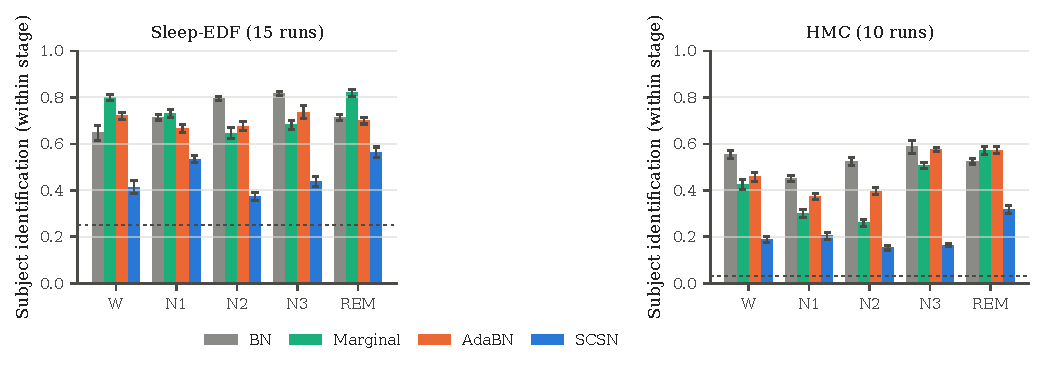
\includegraphics[width=\textwidth]{stage_identity}
\caption{Subject identification within each stage, mean over runs (Sleep-EDF:
fifteen runs; HMC: ten runs), for the uncorrected model (BN), the post-hoc
marginal correction, layerwise AdaBN and SCSN. Error bars are standard errors
over runs; the dashed line is chance. In two HMC runs a held-out recording
contributes fewer than five N3 epochs, so the N3 probe is undefined there;
the HMC N3 mean is over eight runs and the other HMC stages over ten. The
marginal correction moves the within-stage probe little on Sleep-EDF and
partway on HMC; SCSN reduces it in every stage.}
\label{fig:stage-identity}
\end{figure}

The accuracy result follows the same direction but is smaller. On Sleep-EDF
EEGNet SCSN changes accuracy by $+0.002$ [$-0.004$, $+0.009$], $p=0.36$, a
difference indistinguishable from zero; on HMC it gains $+0.019$ [$+0.010$,
$+0.028$], $p=0.0020$, over the uncorrected model, whereas the marginal
correction \emph{loses} $0.023$ [$-0.042$, $-0.005$], $p=0.010$. The HMC
pattern is the one the algebra predicts: marginal adaptation removes the
offset $a_{\cR}$ but adds the stage-mix residual
$\mu_{\mathrm{coh}}-\bar\mu_{\cR}$, which perturbs the logit margin, while
SCSN maps the conditional means back to the prototypes and restores the
margin. The Sleep-EDF cohort is smaller and more homogeneous, and the
accuracy effect there is not detectable.

\subsection{Layerwise AdaBN: what it removes and what it leaves}
\label{sec:adabn}

Layerwise AdaBN is the stronger marginal baseline: it re-estimates the
statistics of every normalization layer on the recording being scored and is
nonlinear. Under the matched probe protocol it changes the overall probe from
$0.715$ to $0.466$ and the within-stage probe from $0.738$ to $0.700$ on
Sleep-EDF EEGNet, and from $0.385$ to $0.212$ and $0.527$ to $0.473$ on HMC
EEGNet. It therefore removes part of the conditional signature as a side
effect, but less than SCSN: the paired difference in within-stage probe
between SCSN and AdaBN is $-0.235$ [$-0.266$, $-0.205$] on Sleep-EDF
($p<10^{-4}$) and $-0.264$ [$-0.278$, $-0.250$] on HMC ($p=0.0020$). On HMC
it also removes less than the post-hoc marginal correction, which moves the
probe from $0.527$ to $0.411$; layerwise statistics replacement is not a
monotone improvement on a single-vector correction.

Figure~\ref{fig:paired} shows the per-run paired structure behind these
averages: every run moves down from the uncorrected model to SCSN, and the
AdaBN points sit between the two.

\begin{figure}[t]
\centering
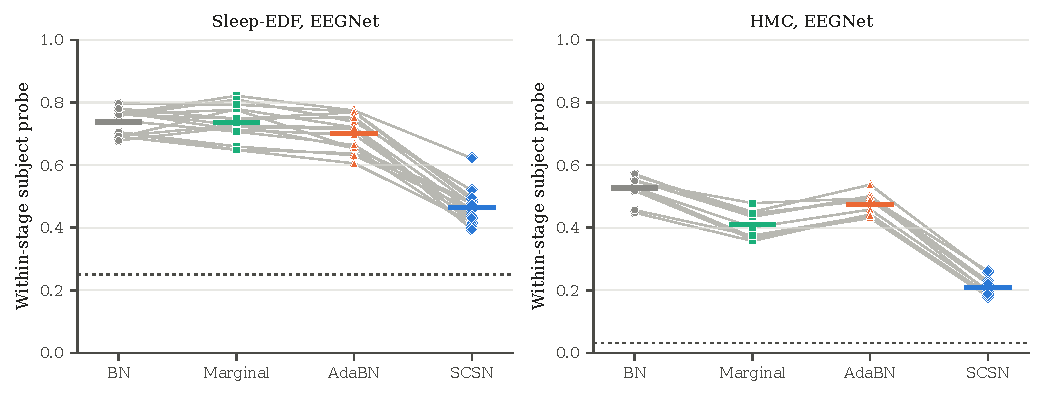
\includegraphics[width=\textwidth]{paired_probe}
\caption{Within-stage subject probe for every run (grey lines), with the arm
mean marked. Left: Sleep-EDF EEGNet, fifteen runs; right: HMC EEGNet, ten
runs. The uncorrected model, the marginal correction, layerwise AdaBN and
SCSN share the checkpoint and the probe subsample of each run.}
\label{fig:paired}
\end{figure}

The residual after AdaBN is informative about its nature. Applying SCSN to the
features produced by layerwise AdaBN changes the within-stage probe by
$-0.0004$ [$-0.0016$, $+0.0009$] ($p=0.85$), a difference that is not
distinguishable from zero: once
every layer has been adapted to the recording, what remains is not a
stage-conditional mean shift, and the correction that targets a mean shift has
nothing to remove. The two methods are therefore alternatives that remove
different components, not two stages of one pipeline. This is consistent with
the layerwise operation: re-estimating the statistics of a batch-normalized
layer rescales and recentres its output per recording, so any additively
stage-conditional component in that output is partly absorbed; what survives
is carried by the higher-order structure of the representation, which a
first-moment correction cannot reach.

\subsection{Accuracy, and where the methods separate}
\label{sec:accuracy}

SCSN is not the most accurate arm on every setting, and we report the
ordering rather than selecting the setting that favors it. On Sleep-EDF
EEGNet, the uncorrected model, the marginal correction, AdaBN and SCSN all
lie within $0.007$ of one another in accuracy, and the paired differences are
not significant (Table~\ref{tab:pairs}). On HMC EEGNet, SCSN is the most
accurate arm, $1.9$ points above the uncorrected model and $4.2$ points above
the marginal correction. On Sleep-EDF SleepCNN, layerwise AdaBN is more
accurate than SCSN by $0.014$ [$-0.033$, $+0.060$], a difference that is not
significant ($p=0.81$), and the uncorrected model is not significantly
different from SCSN. On HMC SleepCNN the three arms are closer: SCSN reaches
$0.712$ against $0.698$ for the uncorrected model and $0.702$ for AdaBN, a
significant gain over the former ($+0.014$ [$+0.006$, $+0.022$], $p=0.004$)
and a margin over the latter that is not significant ($+0.010$ [$-0.001$,
$+0.021$], $p=0.084$). The identity ordering is the
one that is stable across settings: SCSN has the lowest within-stage probe in
every one of the four batch-normalized settings, by margins between $0.27$ and
$0.44$ over the uncorrected model and between $0.24$ and $0.35$ over
layerwise AdaBN.

The Tent baseline is competitive on accuracy and does not remove the
stage-conditional identity. On Sleep-EDF EEGNet, SCSN reaches an accuracy of
$0.784$ against $0.782$ for Tent with the published optimizer on the same
fifteen runs, a difference of $+0.001$ [$-0.006$, $+0.008$], $p=0.85$, while
its within-stage probe is $0.465$ against $0.714$ for Tent, a difference of $-0.249$
[$-0.279$, $-0.220$], $p<10^{-4}$. On HMC EEGNet SCSN is $1.1$ points more
accurate ($+0.011$ [$+0.001$, $+0.021$], $p=0.037$) with a within-stage probe
of $0.209$ against $0.453$. On Sleep-EDF SleepCNN Tent is $1.8$ points more
accurate, a difference that is not significant ($p=0.44$), but its
within-stage probe is $0.858$ against $0.550$. Tent therefore keeps the patient
signature in every setting in which it was run. Tent optimizes a surrogate on the affine
parameters of the normalization layers; it is a batch-normalization method,
and adapting it requires a separate design for group-normalized checkpoints.
The comparison is therefore reported for the batch-normalized setting, and
the group-normalized experiment isolates the applicability of the proposed
correction.

\subsection{Class agreement, calibration and per-stage behavior}
\label{sec:agreement}

An accuracy gain could in principle come from predicting the most frequent
stage more often. The chance-corrected and class-balanced measures in
Tables~\ref{tab:main-eegnet} and~\ref{tab:main-sleepcnn} rule that out: Cohen's
$\kappa$ and the macro-averaged $F_1$ follow accuracy in every arm. Where SCSN
raises accuracy it raises both, by $0.023$ [$+0.012$, $+0.035$] in $\kappa$
and $0.018$ [$+0.008$, $+0.028$] in macro-$F_1$ on HMC EEGNet (paired
$p=0.002$ and $p=0.010$), and by $0.017$ [$+0.006$, $+0.027$] and $0.013$
[$+0.005$, $+0.020$] on HMC SleepCNN ($p=0.014$ and $p=0.006$). On Sleep-EDF the
differences are within noise: $\kappa$ changes by $+0.003$ ($p=0.36$) on
EEGNet and by $-0.005$ ($p=0.62$) on SleepCNN. The HMC gain is therefore
agreement across classes, not a reallocation toward the most frequent stage.

The per-stage recalls show where the accuracy difference comes from. On HMC,
the marginal correction buys N2 recall at the expense of wake and REM: on
EEGNet it raises N2 recall by $0.079$ ($p=0.002$) while lowering wake by
$0.107$ ($p=0.002$) and REM by $0.135$ ($p=0.014$), and on SleepCNN the same
pattern is $+0.063$ for N2 ($p=0.002$) against $-0.174$ for wake ($p=0.002$)
and $-0.036$ for N1 ($p=0.037$), with the losses in N3 and REM in the same
direction but not significant. The residual added by a single-vector correction is the
same for every epoch of the night, so it cannot be stage-specific; on these
checkpoints it shifts the decision toward N2, the most frequent stage. SCSN, which
removes the stage-conditional shift, raises N2 recall by $0.040$ ($p=0.006$)
on EEGNet and by $0.028$ ($p=0.006$) on SleepCNN without a significant loss
in any other stage. Its gain is an improvement of the decision boundary the
head was trained on, not a trade of one stage for another.

Calibration moves against accuracy on the small cohort. On Sleep-EDF EEGNet
SCSN raises the expected calibration error from $0.030$ to $0.044$ ($+0.013$
[$+0.006$, $+0.021$], $p=0.002$). The increase is not specific to SCSN ---
layerwise AdaBN reaches $0.043$ on the same runs --- but it is a cost of
correcting the representation, and it is the reason the limitation in
Section~\ref{sec:discussion} recommends recalibration. On HMC the change is
$+0.006$ ($p=0.049$) on EEGNet and $+0.002$ ($p=0.70$) on SleepCNN, and on the
group-normalized HMC EEGNet SCSN lowers the error by $0.009$ ($p=0.002$).
Conformal coverage is unaffected in every setting because the quantile is
refitted on the calibration split after the correction.

\subsection{Controls}
\label{sec:controls}

Table~\ref{tab:controls} reports the controls on the two EEGNet settings. The
interpolated family shows that identity removal is monotone in $\lambda$:
on Sleep-EDF the within-stage probe falls from $0.673$ at $\lambda=0.25$ to
$0.465$ at $\lambda=1$, while accuracy moves within $0.004$; on HMC it falls
from $0.434$ to $0.209$, while accuracy moves within $0.010$
(Figure~\ref{fig:interp}). The correction therefore buys identity without a
measurable accuracy trade-off on either cohort, and the endpoint $\lambda=0$
is the marginal correction whose within-stage probe is unchanged.

\begin{figure}[t]
\centering
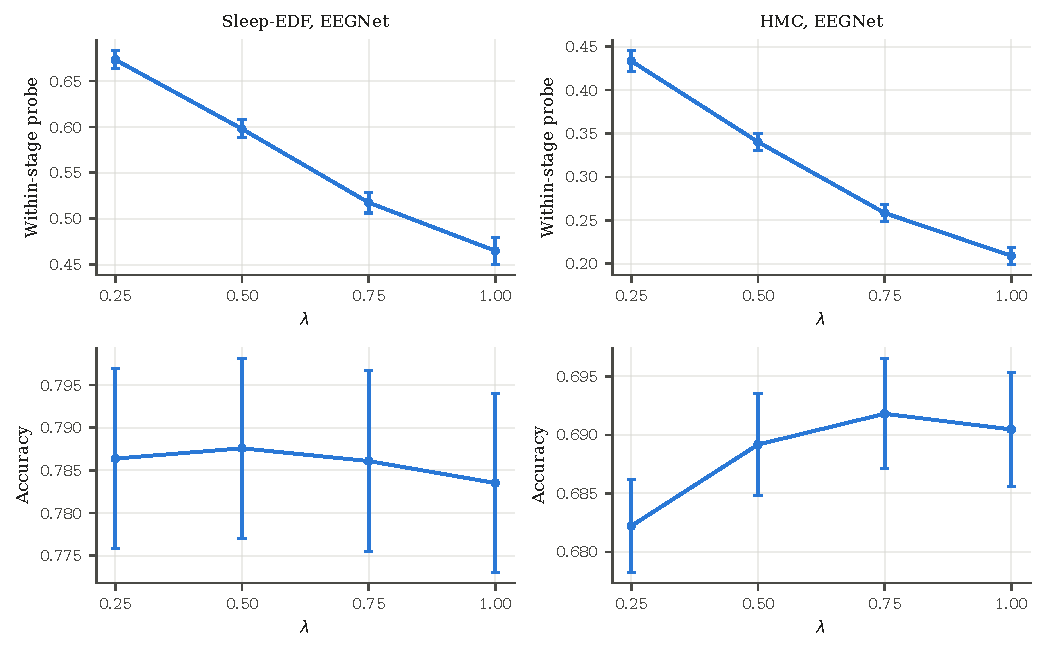
\includegraphics[width=0.85\textwidth]{interpolation}
\caption{The interpolated family: within-stage probe (top) and accuracy
(bottom) as a function of $\lambda$, for Sleep-EDF (left) and HMC (right).
$\lambda=1$ is SCSN, $\lambda\to0$ is the marginal correction. Identity
removal is monotone; accuracy is flat.}
\label{fig:interp}
\end{figure}

\begin{table}[t]
\centering
\caption{Controls on the batch-normalized EEGNet settings: mean accuracy,
within-stage probe, worst-patient conformal coverage and coverage dispersion
over fifteen runs (Sleep-EDF) and ten runs (HMC).}
\label{tab:controls}
\small
\resizebox{\columnwidth}{!}{\begin{tabular}{lrrrrrrrr}
\toprule
 & \multicolumn{4}{c}{Sleep-EDF, EEGNet} & \multicolumn{4}{c}{HMC, EEGNet} \\
\cmidrule(lr){2-5}\cmidrule(lr){6-9}
Arm & Acc & Within & Worst & SD & Acc & Within & Worst & SD \\
\midrule
BN & 0.781 & 0.738 & 0.828 & 0.055 & 0.672 & 0.527 & 0.649 & 0.086 \\
Marginal & 0.777 & 0.735 & 0.838 & 0.047 & 0.648 & 0.411 & 0.599 & 0.096 \\
SCSN-$\lambda_{0.25}$ & 0.786 & 0.673 & 0.837 & 0.049 & 0.682 & 0.434 & 0.665 & 0.079 \\
SCSN-$\lambda_{0.5}$ & 0.788 & 0.598 & 0.845 & 0.043 & 0.689 & 0.340 & 0.680 & 0.072 \\
SCSN-$\lambda_{0.75}$ & 0.786 & 0.518 & 0.851 & 0.039 & 0.692 & 0.258 & 0.678 & 0.069 \\
SCSN ($\lambda=1$) & 0.784 & 0.465 & 0.857 & 0.036 & 0.690 & 0.209 & 0.678 & 0.067 \\
SCSN-$r_1$ & 0.783 & 0.726 & 0.854 & 0.039 & 0.676 & 0.481 & 0.686 & 0.072 \\
SCSN-$r_2$ & 0.783 & 0.695 & 0.857 & 0.033 & 0.685 & 0.435 & 0.678 & 0.069 \\
SCSN-$r_4$ & 0.784 & 0.647 & 0.856 & 0.036 & 0.690 & 0.347 & 0.682 & 0.067 \\
SCSN-orth & 0.781 & 0.792 & 0.828 & 0.055 & 0.672 & 0.559 & 0.649 & 0.086 \\
SCSN-hard & 0.770 & 0.402 & 0.863 & 0.032 & 0.669 & 0.171 & 0.668 & 0.072 \\
SCSN-mismatch & 0.761 & 0.568 & 0.806 & 0.066 & 0.632 & 0.718 & 0.618 & 0.095 \\
\bottomrule
\end{tabular}
}
\end{table}

The rank restriction separates the two effects. Restricting the correction to
the top principal directions of the between-subject, within-stage covariance
removes much less identity than the full correction: $r=4$ leaves a
within-stage probe of $0.647$ on Sleep-EDF and $0.347$ on HMC, against
$0.465$ and $0.209$ for the full correction, and $r=1$ leaves $0.726$ and
$0.481$. Low rank does not buy accuracy: the full correction has the same
accuracy as $r=4$ on both cohorts ($p=0.93$ and $p=1.0$). The conditional
signature is therefore not confined to a few directions, and a practitioner
should not restrict the correction for efficiency.

The orthogonalised control projects each estimated shift off the row space of
the classifier, so the logits are unchanged exactly. Its accuracy is
identical to the uncorrected model on both cohorts, as it must be, and its
within-stage probe is \emph{higher} than the uncorrected model's
($0.792$ against $0.738$ on Sleep-EDF, $0.559$ against $0.527$ on HMC). The
projection removes the component of the shift that the classifier reads and
leaves the component it ignores, which is pure subject information; the
probe sees more of it. This is the clearest evidence that the identity change
in the SCSN arm is not a by-product of a change in predictions.

Two further controls bound the mechanism. Hard pseudo-labels over-correct:
they reduce the within-stage probe slightly more than the soft posterior
($0.402$ against $0.465$ on Sleep-EDF, $0.171$ against $0.209$ on HMC) but
cost $1.3$ and $2.2$ points of accuracy. Mismatched statistics --- applying
the shifts of another recording of the same fold --- remove less identity
($0.568$ and $0.718$ within-stage) and cost accuracy ($-0.022$ and $-0.059$
relative to SCSN, both significant). The effect therefore requires the
recording's own stage-conditional statistics, not merely a perturbation of the
representation.

The shrinkage constant $\lambda_s$ is the only hyperparameter of the
correction, and it is fixed at $10$ throughout. Re-running the SCSN arm with
$\lambda_s\in\{1,100\}$ on the same checkpoints and the same cached
representations, so that only the pseudo-count changes, shows where the value
matters. Between $\lambda_s=1$ and $10$ the arm moves by at most $0.001$ in
accuracy and $0.006$ in the within-stage probe on all four batch-normalized
settings. At $\lambda_s=100$ accuracy is again within $0.004$ points, but the
within-stage probe rises by $0.06$ to $0.11$: the pseudo-count now pulls the
estimated per-stage means towards the cohort prototypes, and the correction
removes less of the signature. The value used is therefore not tuned to the
reported result. Any pseudo-count between one and ten gives the same arm, and
the failure mode at a hundred is over-shrinkage, not sensitivity.

\subsection{Group-normalized stagers}
\label{sec:gn}

The group-normalized checkpoints are the setting in which standard AdaBN
cannot be applied because there is no test-time batch statistic. A bespoke
entropy objective on group-normalization affine parameters is a different
method and is not evaluated here. The post-hoc marginal correction applies,
and it removes the overall probe, but it moves
the within-stage probe by between a tenth and a third of what SCSN removes,
and not consistently in sign: on Sleep-EDF EEGNet it changes the within-stage
probe from $0.638$ to $0.616$ (paired $p=0.030$) and on Sleep-EDF SleepCNN
from $0.832$ to $0.889$, against $0.449$ and $0.583$ under SCSN (paired
changes of $-0.189$ [$-0.205$, $-0.174$] and $-0.248$ [$-0.284$, $-0.213$]).
On HMC EEGNet the uncorrected, marginal and SCSN within-stage probes are
$0.369$, $0.315$ and $0.156$, and on HMC SleepCNN they are $0.663$, $0.745$
and $0.341$; on the latter the marginal correction moves the probe in the
wrong direction (Figure~\ref{fig:gn}).

The accuracy effect points the same way and is smaller than on the
batch-normalized HMC model: SCSN gains $+0.010$ [$+0.005$, $+0.015$]
($p=0.003$) over the uncorrected group-normalized EEGNet and $+0.011$
[$+0.001$, $+0.022$] ($p=0.13$) over SleepCNN on Sleep-EDF, and $+0.016$
[$+0.013$, $+0.019$] and $+0.010$ [$+0.006$, $+0.014$] (both $p=0.0020$)
over HMC EEGNet and SleepCNN; on HMC SleepCNN the marginal correction
\emph{loses} two points. SCSN improves the worst-covered patient on the
Sleep-EDF checkpoints ($0.855$ to $0.864$ on EEGNet and $0.860$ to $0.870$ on
SleepCNN), although the marginal correction improves it there too. On HMC
EEGNet it improves the worst-covered patient from $0.695$ to $0.708$ and the
dispersion from $0.067$ to $0.059$, and on HMC SleepCNN from $0.677$ to
$0.697$ and from $0.070$ to $0.059$, although on both the marginal correction
improves the worst patient further ($0.724$).

\begin{figure}[t]
\centering
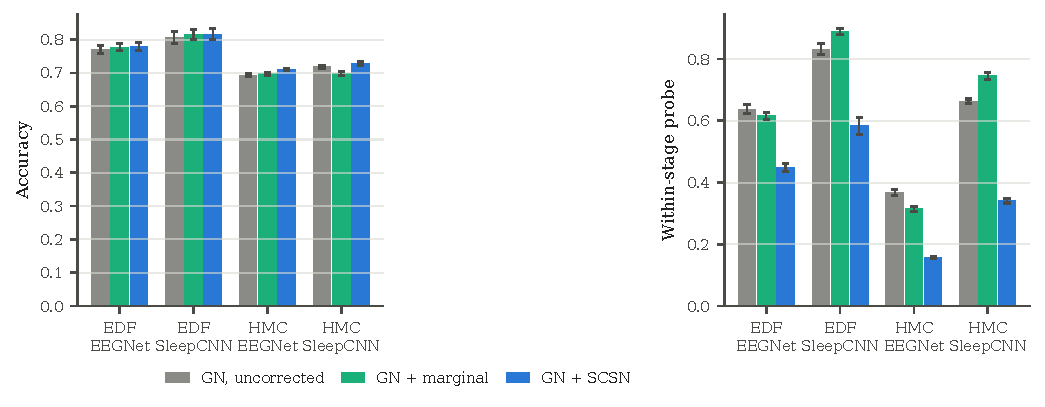
\includegraphics[width=\textwidth]{gn_arms}
\caption{Group-normalized checkpoints: accuracy (left) and within-stage
subject probe (right) for the uncorrected model, the post-hoc marginal
correction and SCSN. Error bars are standard errors over runs. The marginal
correction moves accuracy and the overall probe but barely moves the
within-stage probe; SCSN reduces it.}
\label{fig:gn}
\end{figure}

The result is the one the normalization argument predicts.
Group normalization removes the batch from the computation, so the
representation of an epoch depends only on that epoch; it does not follow
that the representation is free of the recording. The network that follows
the normalized layers maps the remaining recording-dependent variation into
the penultimate space, and a linear probe recovers the patient from it. Among
the statistics-replacement approaches compared here, SCSN is the only
stage-aware correction; it works without a batch statistic, optimizer, or
weight update.

\subsection{Patient-level conformal reliability}
\label{sec:coverage}

At $\alpha=0.1$ every arm covers at close to the nominal rate on average, and
the average hides the patient dependence. On Sleep-EDF EEGNet the
uncorrected model has a per-patient coverage standard deviation of $0.055$
and a worst-covered patient of $0.828$; the marginal correction improves them
to $0.047$ and $0.838$, and SCSN to $0.036$ and $0.857$. On HMC EEGNet the
same ordering holds against the uncorrected model: SCSN improves the
dispersion from $0.086$ to $0.067$ and the worst patient from $0.649$ to
$0.678$, while the marginal correction \emph{worsens} both ($0.096$ and
$0.599$). Layerwise AdaBN also improves the worst-covered patient over SCSN
in both settings ($0.866$ against $0.857$ on Sleep-EDF; $0.698$ against
$0.678$ on HMC), and its dispersion is smaller on Sleep-EDF ($0.028$ against
$0.036$) and comparable on HMC ($0.069$ against $0.067$). We report that
rather than the comparison that favors the method: on a batch-normalized
model, re-estimating every layer is a strong reliability intervention. On the
group-normalized checkpoints, where standard AdaBN is unavailable, SCSN
improves both quantities over the uncorrected model
(Table~\ref{tab:main-eegnet}).

Figure~\ref{fig:coverage} shows the empirical distribution of per-patient
coverage. Below the nominal level the uncorrected curve carries more mass
than the SCSN curve, and the marginal curve is the worst of the three on HMC;
above the nominal level the SCSN curve is the steeper one, so the shortfall of
the patients that do fall short is smaller. The review workload moves with the
sets: on Sleep-EDF EEGNet the fraction of multi-stage prediction sets falls
from $0.750$ to $0.729$ under SCSN and to $0.741$ under the marginal
correction.

\begin{figure}[t]
\centering
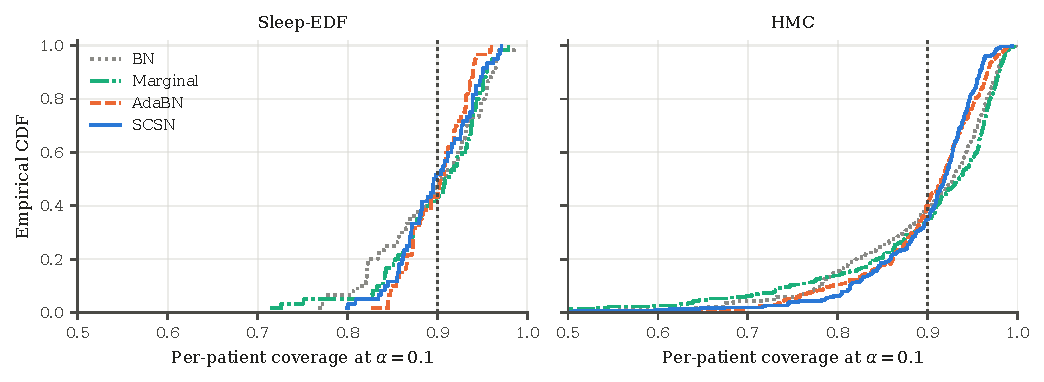
\includegraphics[width=\textwidth]{coverage_ecdf}
\caption{Empirical distribution of per-patient conformal coverage at
$\alpha=0.1$, pooled over runs. The dashed line is the nominal level. The
uncorrected model has more mass below the nominal level; the marginal
correction moves the distribution in the wrong direction on HMC, and SCSN
moves it in the right direction on both cohorts.}
\label{fig:coverage}
\end{figure}

\subsection{Transfer to a second centre, and the precondition of the method}
\label{sec:transfer}

A checkpoint trained on Sleep-EDF and never shown an HMC epoch is evaluated on
all $137{,}243$ HMC epochs under the source statistics, the post-hoc marginal
correction, SCSN, layerwise AdaBN and SCSN stacked on AdaBN
(Table~\ref{tab:cross}). This is a transfer across population, montage,
equipment, sampling rate and scoring manual, not merely across patients.

Under the source statistics the model reaches an accuracy of $0.475$ with a
worst-recording accuracy of $0.128$. The marginal correction raises accuracy
to $0.505$; layerwise AdaBN raises it to $0.553$ and the worst recording to
$0.214$. SCSN reaches $0.489$, below both. The oracle variant, which uses the
true stages to estimate the shifts, reaches $0.727$: the estimator is not the
limitation, the posterior is. When the source model is applied to a cohort it
was not trained on, its posterior is weak, the stage-conditional means
estimated from it are dominated by the prior and the recording offset, and the
correction behaves like the marginal one. SCSN should therefore not be applied
blindly across cohorts; the precondition is a posterior informative enough to
index the stages, and it can be checked on the unlabeled night before the
correction is applied.

\begin{table}[t]
\centering
\caption{Cross-cohort transfer: a Sleep-EDF checkpoint evaluated on all HMC
epochs. ``Worst'' and ``SD'' are the minimum and standard deviation of
per-recording accuracy. The group-normalized checkpoints have no statistics to
replace and are not part of this table.}
\label{tab:cross}
\small
\resizebox{\columnwidth}{!}{\begin{tabular}{lrrr}
\toprule
 & \multicolumn{3}{c}{EEGNet} \\
\cmidrule(lr){2-4}
 & Acc & Worst & SD \\
\midrule
Cohort statistics & 0.475 & 0.128 & 0.150 \\
Marginal & 0.505 & 0.115 & 0.143 \\
SCSN & 0.489 & 0.114 & 0.156 \\
SCSN-$\lambda_{0.5}$ & 0.497 & 0.113 & 0.152 \\
AdaBN & 0.553 & 0.214 & 0.134 \\
AdaBN + SCSN & 0.555 & 0.204 & 0.139 \\
SCSN (oracle labels) & 0.727 & 0.245 & 0.120 \\
\bottomrule
\end{tabular}
}
\end{table}

\begin{figure}[t]
\centering
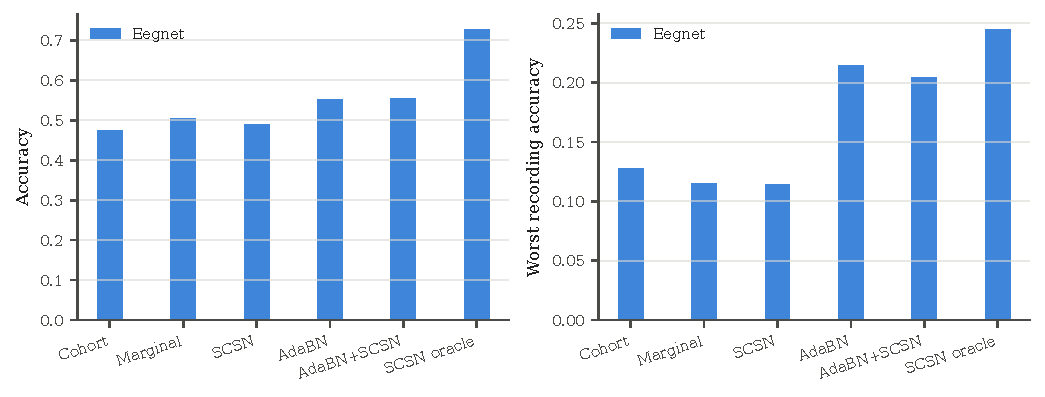
\includegraphics[width=\textwidth]{cross_cohort}
\caption{Cross-cohort accuracy (left) and worst-recording accuracy (right) for
the transferred checkpoint. The oracle uses the true stages; the gap between
it and SCSN is the cost of the weak target posterior.}
\label{fig:cross}
\end{figure}

Two caveats bound this experiment. Every arm is evaluated on a single
checkpoint, and no subject probe is computed on the transferred
representation, so the section speaks to accuracy and per-recording spread,
not to identity.
It shows that the intervention travels with the model to an unseen centre only
when the posterior does; the within-cohort experiments of
Sections~\ref{sec:scsn-identity}--\ref{sec:adabn} are what show that the
identity decomposition is the same there.
